%# -*- coding: utf-8-unix -*-
%%==================================================
%% chapter02.tex for SJTU Master Thesis
%% based on CASthesis
%% modified by wei.jianwen@gmail.com
%% Encoding: UTF-8
%%==================================================


\chapter{基于规范的入侵检测设计}
\label{chap:spec detection}

\section{引言}
\label{sec:intro}
在上一章节中我们讨论了如何对控制器与物理设备交互的输入输出信号进行检测保护,防御对象系统主要是故障和异常数据注入攻击,为此我们还专门设计错误序列注入攻击对其进行仿真验证。但是对控制器本身尤其是PLC这种可编程控制器,由于它们在整个控制系统中发挥至关重要的作用,近年来正成为对物理设备损坏性攻击的有吸引力的目标。最为典型的Stuxnet病毒可以向PLC上传恶意代码,以物理损坏他们控制的离心机。更有研究发现,PLC控制器不仅容易被端口扫描,而且还可以被修改控制系统特定协议和被访问诊断系统。这些易受攻击的互联网控制器被计算机搜索引擎暴露,例如Shodan。所以对可编程控制器本身控制程序和指令的保护并使其免受恶意代码注入的保护也同样重要。本章我们提出了基于规范的的入侵检测来应对控制器的恶意代码注入攻击,只有经过验证合法的程序和指令才能操作系统或控制服务器上传到指定的可编程控制器设备中。

\section{入侵检测方案概述}
\label{sec:list}

本文我们采用PLC作为待检测可编程控制器,检测机制作为外部单独的功能处理器BITS(Bump-in-the-wire)模式放置在控制系统网络和PLC之间。对于任何等待上传到工业设备的PLC代码,将被拦截并验证由过程安全工程师定义的一整套安全规范(safety properties),安全特性的示例包括数字设备参数(例如最大驱动速度和加速度)和安全互锁的界限并确保不发生物理上冲突的事件。图\ref{fig21}展示了基于规范入侵检测机制的基本过程,首先将PLC代码(IL code)格式化整理并通过IL2boolIL算法转换为中间语言,我们定义为布尔逻辑指令表代码(Boolean IL code),旨在使抽象程序逻辑清晰更具一般性。然后布尔逻辑指令表代码通过模板实例化(Template Instantiate
)过程被迭代地执行将通用模板代码实例化为验证工具NuSMV输入程序。前面两步是对PLC程序的形式化建模过程,接下来我们给出验证过程。我们通过将得到的形式化代码模型(NuSMV code)输入到验证工具NuSMV逐个地检查我们的安全规范。每个布尔规范表示有限状态机中的安全属性是真还是假,如果存在任何可达的路径其属性为假,则会给出相应的反例并证明存在安全违规不能上传到PLC设备中。

\begin{figure}[!htb]
		\centering
		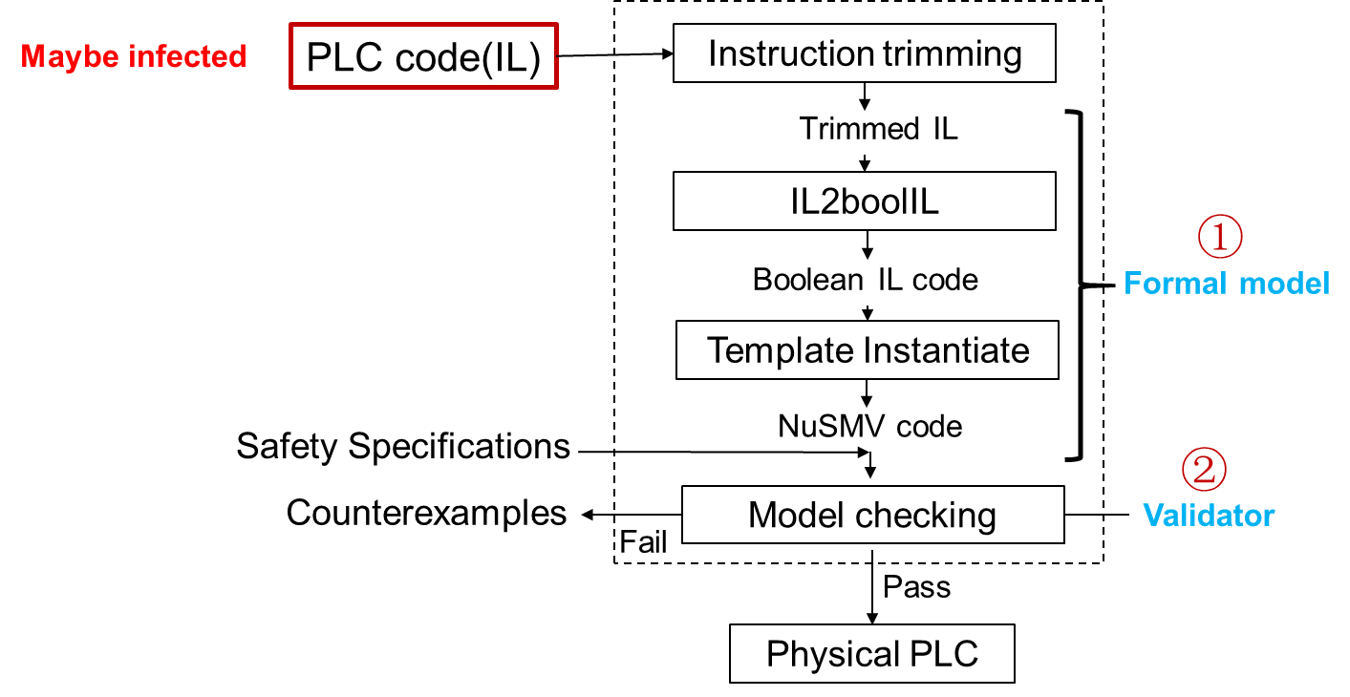
\includegraphics[scale=0.49]{spec/flowchart_spec.png}
		\caption{基于规范的入侵检测流程图}
		\label{fig21}
	\end{figure}

\section{系统建模和入侵检测设计}
\label{sec:matheq}


\section{实验仿真}
\label{sec:insertimage}

\section{本章小结}
\label{sec:insertimage}

